% ===========================================================================
%  utente/01-primi-passi/00-capitolo.tex
% ===========================================================================
\chapter{Primi passi}\label{cap:primi-passi}

\begin{attenzione}{I numeri nelle schermate sono inventati}
Tutte le immagini di questo manuale sono state fatte su un'installazione con
\emph{dati di esempio}: serie generate al calcolatore, non prezzi reali e non
risultati di strategie. Servono a mostrare dove si trovano le cose. Nessuno
Sharpe, nessun rendimento e nessun drawdown di queste pagine significa
qualcosa.
\end{attenzione}

\section{Che cosa fa Lyra}\label{sez:cosa-fa}

Tre cose, in quest'ordine:

\begin{enumerate}
  \item \textbf{Costruire} una strategia di investimento --- scrivendola,
        disegnandola a blocchi, o descrivendola a parole.
  \item \textbf{Provarla} sui dati del passato, con i costi, e vedere come si
        sarebbe comportata.
  \item \textbf{Farla girare} su un conto vero, quando regge.
\end{enumerate}

\noindent
Le strategie si possono anche combinare fra loro, e si possono comprare e
vendere fra utenti nel \voce{Marketplace}. Questo manuale segue lo stesso
ordine: un capitolo per zona dell'applicazione.

\figuraTikz{flusso-utente}
  {Le zone dell'applicazione, nell'ordine in cui si usano. La freccia che
   torna indietro è la parte più frequente del lavoro.}
  {flusso-utente}

\section{Il menu}\label{sez:menu}

La barra a sinistra è sempre presente. Si allarga passandoci sopra con il
mouse e mostra i nomi delle voci.

\begin{figure}[htbp]
  \centering
  \setlength{\fboxsep}{0pt}\setlength{\fboxrule}{0.5pt}%
  {\color{lyraGrigioChiaro}\fbox{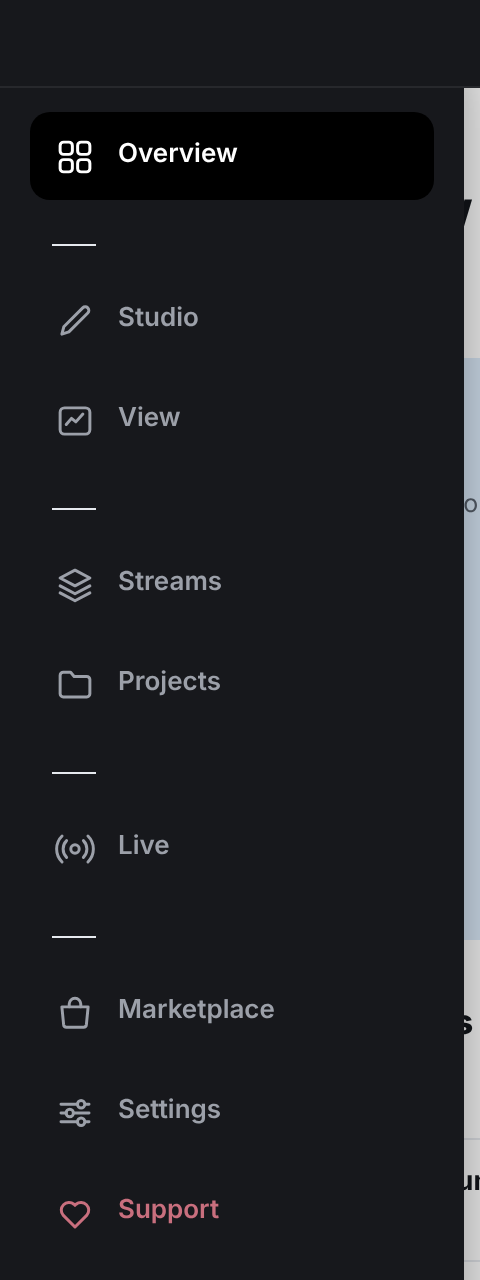
\includegraphics[width = 0.26\linewidth]
    {figure/schermate/menu.png}}}
  \caption{Il menu, allargato. Le voci sono in quattro gruppi: costruire,
           provare, far girare, comunità.}
  \label{fig:menu}
\end{figure}

\begin{center}
\begin{tabular}{@{}L{26mm}L{18mm}L{90mm}@{}}
\toprule
\textbf{Voce} & \textbf{Gruppo} & \textbf{A che serve} \\
\midrule
\rigaTenue
\voce{Overview} & Workspace & La schermata iniziale: come va tutto, in una
  pagina. \\
\voce{Studio} & Build & Dove si costruiscono le strategie. \\
\rigaTenue
\voce{View} & Build & I grafici con sopra quello che la strategia ha fatto. \\
\voce{Streams} & Test & I risultati: una scheda per strategia. \\
\rigaTenue
\voce{Projects} & Test & Le combinazioni di più strategie. \\
\voce{Live} & Run & Il collegamento a un conto vero. \\
\rigaTenue
\voce{Marketplace} & Community & Comprare e vendere strategie. \\
\voce{Settings} & Settings & Dati, parametri, regimi di mercato. \\
\bottomrule
\end{tabular}
\end{center}

\begin{nota}{In alto a destra}
La lente cerca in tutta l'applicazione; la campanella mostra i lavori
conclusi e i messaggi; il sole cambia fra chiaro e scuro; l'ultima voce è
l'accesso al proprio conto.
\end{nota}

\section{Serve un account?}\label{sez:account-serve}

Per costruire, provare e far girare le strategie, \textbf{no}:
l'applicazione gira sul computer di chi la usa e non chiede nulla.

Serve un account solo per le zone che passano dalla rete: il
\voce{Marketplace}, i messaggi, il profilo, l'abbonamento. Aprendo una di
quelle senza aver fatto l'accesso, l'applicazione lo dice e offre di farlo.

\section{L'ordine in cui si lavora}\label{sez:ordine}

\begin{pratica}{Dal nulla al primo risultato}
\begin{enumerate}
  \item \percorso{Settings \freccia Data}: scaricare i dati. Senza, tutte le
        pagine sono vuote --- non è un errore, non c'è niente da mostrare.
  \item \percorso{Streams \freccia Run backtest}: scegliere una strategia e
        premere \pulsante{Run backtest}.
  \item Aspettare. Il lavoro gira in sottofondo e la campanella avvisa alla
        fine; nel frattempo si può usare il resto dell'applicazione.
  \item \voce{Streams}: il risultato è comparso come scheda.
  \item \voce{Projects}: combinare due o più risultati.
  \item \voce{Live}: collegare un broker, quando si è pronti.
\end{enumerate}
\end{pratica}
